% Matlab 的程序调试及其他功能

\pentry{Matlab 的文件, 程序结构和函数\upref{MatSrt}}

\subsection{程序调试}
\begin{figure}[ht]
\centering
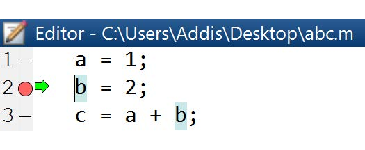
\includegraphics[width= 6cm]{./figures/Matlab3.pdf}
\caption{在行首设置 Breakpoint}\label{Matlab_fig3}
\end{figure}

若要调试程序,可选择一行代码并单击该行前面的横线,这时会出现红色圆点 Breakpoint (\autoref{Matlab_fig3}),程序运行到 Breakpoint 会暂停.

此时要查看变量情况,可通过 Workspace 查看各个变量的情况,也可用光标悬停在某个变量上.还可以用 Command Window 改变某些变量的值,或画图等.在这种调试状态下,也可以通过 Edit 菜单中的一些按钮控制接下来程序如何运行(\autoref{Matlab_fig4}).
\begin{figure}[ht]
\centering
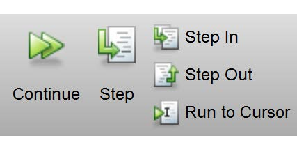
\includegraphics[width= 5cm]{./figures/Matlab4.pdf}
\caption{Step 菜单}\label{Matlab_fig4}
\end{figure}
其中“Continue”(快捷键 F5)是继续运行直到下一个 Breakpoint 或结束.“Step”(F10)是运行到下一行,“Step In”(F11)是进入子程序并暂停,“Step Out”是运行完当前子程序并回到子程序被调用的地方.“Run to Cursor”是运行到光标所在处.

\subsection{分节}
在行首用两个百分号“\texttt{\%\%}” 可以对代码进行分节(\autoref{Matlab_fig5}).这样做一是可以使代码结构更清晰,二是可以单独选择某一节运行(Edit 菜单中的“Run Section”按钮).
\begin{figure}[ht]
\centering
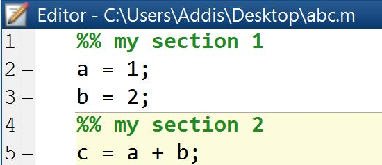
\includegraphics[width= 6cm]{./figures/Matlab5.pdf}
\caption{代码分节}\label{Matlab_fig5}
\end{figure}

\subsection{工具箱(Toolbox)}
在购买和安装 Matlab 软件时,可以选择各种各样的工具箱,常用的工具箱有曲线拟合(Curve Fitting,从离散的数据点得到一条曲线),图像处理(Image Processing,图像变换,增强,降噪,二值化等),图像获取(Image Acquisition,从相机获取图像),Matlab 编译器(MATLAB Compiler,编译代码,提高运行速度).注意使用了工具箱功能的代码在没有工具箱的 Matlab 软件上将无法运行.

\subsection{Matlab Online}
具有 Matlab 的基本功能,和类似于软件的界面,需要购买了正版 Matlab 的 Matlab 账号登录(学生账号也可以).若账号购买了工具箱(Toolbox),也可以使用对应的工具箱.本书官网提供免费的 Matlab 账号供读者试用和体验 Matlab Online,网址见本书封面或前言.



